\documentclass{beamer}
\usepackage[utf8]{inputenc}
\usetheme{Copenhagen}
\usepackage[english]{babel}
\usepackage{multirow}
%\usepackage{estilo-apuntes}
\usepackage{braids}
\usepackage[]{graphicx}
\usepackage{rotating}
\usepackage{pgf,tikz}
\usepackage{pgfplots}
\usepackage{tikz-cd}
\usetikzlibrary{arrows}
\usetikzlibrary{cd}
%\usepackage[T1]{fontenc}
%\usepackage{CJKutf8}
%\usepackage{CJK}
%\usetikzlibrary{babel}
%\usepackage{kotex}
\pgfplotsset{compat=1.13}
\usetikzlibrary{decorations.shapes}
\pgfkeyssetvalue{/tikz/braid height}{1cm} %no parece hacer nada
\pgfkeyssetvalue{/tikz/braid width}{1cm}
\pgfkeyssetvalue{/tikz/braid start}{(0,0)}
\pgfkeyssetvalue{/tikz/braid colour}{black}

\theoremstyle{definition}

\newtheorem{teorema}{Teorema}
\newtheorem{defi}[teorema]{Definición}
\newtheorem{prop}[teorema]{Proposición}
\newtheorem{ej}[teorema]{Ejemplo}

\newcommand{\Z}{\mathbb{Z}}
\newcommand{\C}{\mathbb{C}}
\newcommand{\D}{\mathbb{D}}
\providecommand{\gene}[1]{\langle{#1}\rangle}


\addtobeamertemplate{navigation symbols}{}{%
    \usebeamerfont{footline}%
    \usebeamercolor[fg]{footline}%
    \hspace{1em}%
    \insertframenumber/\inserttotalframenumber
}
\setbeamercolor{footline}{fg=black}
\setbeamerfont{footline}{series=\bfseries}

%-----------------------------------------------------------

\title{Computation of words satisfying the “rhythmic oddity property”}
\author{Javier Aguilar Martín}
\institute{Universidad de Sevilla}
\date{}
 
\begin{document}
\frame{\titlepage}
%\begin{frame}
%
%
%\title[About Beamer] %optional
%{About the Beamer class in presentation making}
% 
%\subtitle{A short story}
% 
%\author[Arthur, Doe] % (optional, for multiple authors)
%{A.~B.~Arthur\inst{1} \and J.~Doe\inst{2}}
% 
%\institute[VFU] % (optional)
%{
%  \inst{1}%
%  Faculty of Physics\\
%  Very Famous University
%  \and
%  \inst{2}%
%  Faculty of Chemistry\\
%  Very Famous University
%}
% 
%\date[VLC 2013] % (optional)
%{Very Large Conference, April 2013}


%\end{frame}
\setbeamercovered{highly dynamic}

\newcounter{saveenumi}
\newcommand{\seti}{\setcounter{saveenumi}{\value{enumi}}}
\newcommand{\conti}{\setcounter{enumi}{\value{saveenumi}}}

\resetcounteronoverlays{saveenumi}


\section{Introduction}

\begin{frame}
\frametitle{Introduction}
Aka Pygmies rythmic pattern: 32222322222
\begin{figure}[h!]
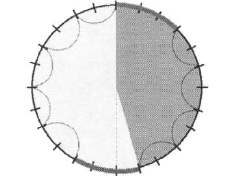
\includegraphics[scale=0.7 ]{circulo}
\caption{No breaking point giving two parts of equal length.}
\end{figure}
\end{frame}

%\begin{frame}
%\frametitle{Concatenación}
%\begin{figure}[h!]
%\includegraphics[scale=0.5]{Imagenes/Diapconca}
%\caption{Concatenación de trenzas.}
%\end{figure}
%Esta operación induce un producto entre las clases de homotopía.
%\end{frame}



\section{The rythmic oddity property}

\begin{frame}
\frametitle{Words}
\begin{itemize}
\item<1-> Alphabet $A=\{2,3\}$, $A^*=$words over $A$, $\varepsilon=$empty word. 
\item<2-> $A^*$ is a monoid under concatenation.
\item<3-> For $w\in A^*$, $|w|=$lenght of $w$, $|w|_x=$number of symbols in $w$ equal to $x$.
%\item<4-> $u$ is a \textbf{prefix} of $w$ is $w=uy$ for some $y\in A^*$.
%\item<5-> $u$ is a \textbf{suffix} of $w$ is $w=yu$ for some $y\in A^*$.
\end{itemize}
\end{frame}

\begin{frame}
\frametitle{Cyclic shifts}
Let $\delta$ be a permutation of $A^*$ defined by $\delta(\varepsilon)=\varepsilon$, $\delta(au)=ua$ for $a\in A$ and $u\in A^*$.

\begin{itemize}
\item<1-> The \textbf{cyclic shifs} of $w$ are the words of the form $\delta^k(w)$ for any integer $k$.
\end{itemize} 

\only<2->{\begin{example}
$w=2223$ has cyclic shifts $2223$, $2232$, $2322$, $3222$.  
\end{example}}

\begin{itemize}
\item<3-> The \textbf{height} is a morphism $h:A^*\to\mathbb{N}$ defined by $h(u)=$sum of its symbols.
\end{itemize} 
\end{frame}

\begin{frame}
\frametitle{The rythmic oddity property}
\begin{alertblock}{Definition}
A word $w$ satisfies the \textbf{rythmic oddity property} if and only if
\begin{itemize}
\item $h(w)$ is even and
\item no cyclic shift of $w$ can be factorized into words $uv$ such that $h(u)=h(v)$. 
\end{itemize}
\end{alertblock}
\only<2->{\begin{example}
For the Aka Pygmies $32222322222$, $h(w)=24$ and any factorization of cyclic shifts gives $h(u)=11$ and $h(v)=13$ or viceversa. 
\end{example}}
\end{frame}

%\begin{frame}
%\begin{block}{Proposition 1}
%If $w$ satisfies the rythmic oddity property, then at least one of the following conditions is
%satisfied:
%\begin{itemize}
%\item there exists a unique pair $(u,v)$ with $h(v)=h(u)+2$ such that $w=uv$, or 
%\item there exists a unique pair $(u,v)$ with $h(v)=h(u)+2$ such that$w=vu$. 
%\end{itemize}
%\end{block}
%
%
%
%\end{frame}
%\begin{frame}
%\frametitle{Asymmetric pairs}
%A pair $(u,v)$ is called \textbf{asymmetric} if no pair of prefixes $(u',v')$ exists such that $h(v')=h(u')+1$. 
%
%\begin{example}
%$(33222,32322)$ is an asymmetric pair but $(3322,32232)$ is not because $h(322)=h(33)+1$. 
%\end{example}
%\begin{block}{Proposition 2}
%A word $w$ satisfies the rythmic oddity property if and only if there exists an assymetric pair $(u,v)$ such that $w=uv$ or $w=vu$ with $h(v)=h(u)+2$. 
%\end{block}
%\end{frame}


\section{Key construction}

\begin{frame}
\frametitle{Key construction}
\begin{itemize}
\item<1-> Consider $a,b:A^*\times A^*\to A^*\times A^*$ defined by $a(u,v)=(3u,3v)$ and $b(u,v)=(v,2u)$. 
\item<2-> Let $B=\{a,b\}$ and consider the free monoid $B^*$.
\item<3-> Let $D=\{w=uv, \exists\alpha\in B^*, |\alpha|_b$ odd, $(u,v)=\alpha(\varepsilon,\varepsilon)\}\subset A^*$
\end{itemize}
%\begin{block}{Proposition 3}
%The set of asymmetric pairs is equal to the smallest set of pairs of words containing $\varepsilon\times A^*$ and $A^*\times\varepsilon$ and closed under $a$ and $b$. 
%\end{block}
\only<4->{\begin{alertblock}{Lemma}
A word $w$ satisfies the rythmic oddity property if anf only if $w$ is a cyclic shift of an element of $D$. 
\end{alertblock} }
\only<5>{For $w\in D$ define $f:D\to B^*$ by $f(w)=\alpha$ ($\alpha$ is unique). $f$ is injective and $f(D)$ consists of the words of $\alpha\in B^*$ with $|\alpha|_b$ odd. }
\end{frame}


%\begin{frame}
%
%
%\begin{block}{Proposition 4}
%Let $(u,v)=\alpha(\varepsilon,\varepsilon)$ for $\alpha\in B^*$. If $|\alpha|_b$ is even, then $h(v)=h(u)$, and if $|\alpha|_b$ is even, then $h(v)=h(u)+2$. 
%\end{block}
%\begin{block}{Proposition 5}
%If $|\alpha|_b$ is even, then $\alpha(r,s)=\alpha(\varepsilon,\varepsilon)(r,s)$, and if $|\alpha|_b$ is odd, then $\alpha(r,s)=\alpha(\varepsilon,\varepsilon)(s,r)$.
%\end{block}
%
%{
%\setbeamercolor{block title}{bg=green, fg=white}
%\begin{block}{Corollary 6}
%A word $w$ satisfies the rythmic oddity property if and only if there exists a word $\alpha\in B^*$ with $|\alpha|_b$ being odd, such that $w=uv$ or $w=vu$ with $(u,v)=\alpha(\varepsilon,\varepsilon)$.
%\end{block}
%}
%\end{frame}
%\begin{frame}






%\begin{block}{Proposition 7}
%For any $w,w'\in D$, $f(w')$ is a cyclic shift of $f(w)$ if and only if $w'$ is a cyclic permutation of $w$.
%\end{block}
%\end{frame}

\begin{frame}
\begin{example}
Computation of $f(w)$ where $w=332232322$. Factorization $w=uv$ such that $h(v)=h(u)+2$ gives $u=3322$ and $v=32322$. Then 
\begin{align*}
(u, v) &= (3322, 32322)\\
&= a(322, 2322)\\
&= ab(322, 322)\\
&= aba(22, 22)\\
&= abab(2, 22)\\
&= ababb(2, 2)\\
&= ababbb(\varepsilon, 2)\\
&= ababbbb(\varepsilon, \varepsilon)\Rightarrow f(332232322)=ababbbb
\end{align*}
%which gives $f(332232322)= ababbbb$.
\end{example}
\end{frame}
\section{Lyndon words}
\begin{frame}
\frametitle{Lyndon words}
\begin{itemize}
\item The \textbf{conjugacy} relation on words is the equivalence
between words being cyclic shifts of one another.
\item<2-> \textbf{Lyndon words} are defined as
minimal elements in the conjugacy classes regarding
the lexicographic order, with the additional condition
that they are primitive (not power of another word).
\item<3-> Lyndon words of length $n>1$ are
obtained by concatenating Lyndon words of length $p$
and $q$ with $n = p+q$.

\only<4>{\begin{example}
$$aababb=(aab)(abb)$$
\end{example}} 
\end{itemize}

\end{frame}

\section{Algorithm}
\begin{frame}
\frametitle{Algorithm}
\begin{itemize}
\item<1->  Let $a$ be the smallest
letter of the ordered alphabet $\Sigma$ and $M$ be the largest one.
\item<2-> For every $x\in \Sigma\setminus\{M\}$, $s(x)$ is the
letter that immediately larger than $x$. 
\item<3-> Denote by
$w[1...n]$ an array of letters of dimension $n$.
\end{itemize}


%AQUÍ VIENE EL ALGORITMO PARA CALCULAR PALABRAS DE LYNDON Y LA REFERENCIA 8 DONDE SE EXPLICA, Y DE HECHO VIENE LO DE ESTE ARTÍCULO
%\url{http://ehess.modelisationsavoirs.fr/marc/publi/softcomputing/5000387periodicity.pdf}

\end{frame}

\begin{frame}

\textbf{Computation of Lyndon words of length $\leq n$}

\begin{figure}
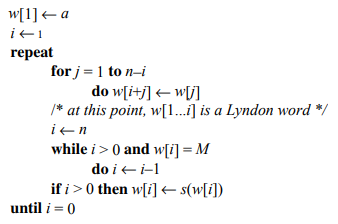
\includegraphics[scale=0.8]{algoritmo}
\end{figure}

\end{frame}

\begin{frame}
\textbf{Computation of words satisfying the rythmic oddity property}
\begin{itemize}
\item<2-> Apply the previous algorithm to $\Sigma=B$.
\item<3-> Take only those words with an odd number of symbols equal to $b$. 
\item<4-> To recover the words in $A^*$ evaluate each solution on $(\varepsilon,\varepsilon)$. 
\end{itemize}
\end{frame}
\section{Counting the solutions}



\begin{frame}
\frametitle{Counting the solutions}
\begin{itemize}


\item
 Let $n_2$ and $n_3$ be the number of two- and three-unit
elements of a solution. 

\item<2->Let $X(p)$ be the number of words $w$ satisfying the
rhythmic oddity property up to a cyclic shift, where $p$
is the length of $f (w)$.
\end{itemize}

\only<3>{\begin{alertblock}{Proposition}
If $n_3 = 2j$ is a power of 2, one has
$$X(p)=\frac{1}{p}\binom{p}{j}.$$
\end{alertblock}}
\end{frame}

\begin{frame}[fragile]
\begin{figure}[h!]
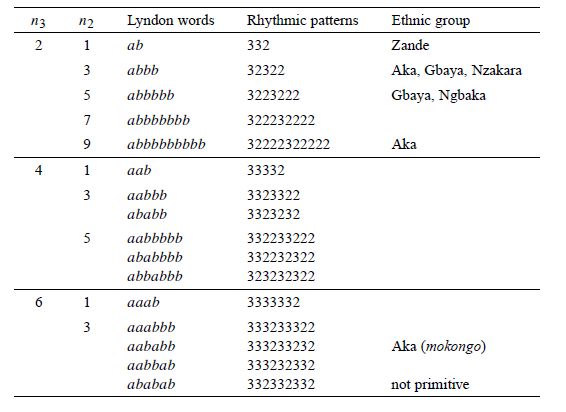
\includegraphics[scale=0.5]{tabla}
\end{figure}

\end{frame}







%\begin{frame}[fragile]
%\frametitle{Generadores del grupo de trenzas puras}
%%\begin{figure}[h!]
%%\includegraphics[scale=0.5]{Imagenes/birman}
%%\caption{Generador de Birman $A_{ij}$.}
%%\end{figure}
%\begin{figure}[h!]
%\centering
%\tikzset{decorate sep/.style 2 args=
%{decorate,decoration={shape backgrounds,shape=circle,shape size=#1,shape sep=#2}}}
%\resizebox{9cm}{4cm}{%
%\begin{tikzpicture}
%
%\node[anchor=south] at (0,2.1) {$j$};
%\foreach \x in {-7,-4,-2,-1,1,4}{
%\draw[white,double=black,very thick,-] (\x,-2) -- (\x,2);
%}
%\draw[white,double=black,very thick,-] (-3,0) -- (-3,2);
%\draw[smooth,white,double=black,line width=2mm,-] plot[variable=\x,domain=-2:2] ({-3.5*exp(-1.4*\x*\x)},{\x});
%\draw[white,double=black,very thick,-] (-3,-2) -- (-3,0);
%\node[anchor=south] at (-3,2.1) {$i$};
%\draw[decorate sep={0.5mm}{9mm},fill] (-6.5,0) -- (-4.5,0);
%\draw[decorate sep={0.5mm}{9mm},fill] (1.5,0) -- (3.5,0);
%\draw[-] (-8,2) -- (5,2);
%\draw[-] (-8,-2) -- (5,-2);
%\end{tikzpicture}
%}
%\caption{Generador de Birman $A_{ij}$.}
%\end{figure}
%\end{frame}


%\begin{frame}
%\frametitle{Automorfismos del grupo libre}

%\begin{figure}[h!]
%\includegraphics[scale=0.7]{Imagenes/Disco.png}
%\caption{Los lazos $x_1,\dots,x_n$ son generadores de $\pi_1(\D_n)\cong F_n$.}
%\end{figure}
%\end{frame}

%\begin{frame}
%\begin{align*}
%\rho: & B_n \to Aut(F_n)\\
%      & \beta\ \ \mapsto\ \ \rho_\beta
%\end{align*}
%
%$$\rho_{\sigma_i}(x_i)=x_{i+1},\quad \rho_{\sigma_i}(x_{i+1})=x_{i+1}^{-1}x_ix_{i+1},\quad \rho_{\sigma_i}(x_j)=x_j\ (j\neq i,i+1)$$
%
%$$\rho^{-1}_{\sigma_i}(x_i)=x_ix_{i+1}x_i^{-1},\quad \rho^{-1}_{\sigma_i}(x_{i+1})=x_i,\quad \rho^{-1}_{\sigma_i}(x_j)=x_j\ (j\neq i,i+1)$$
%\end{frame}

%\begin{frame}
%\begin{figure}[h!]
%\includegraphics[scale=0.5]{Imagenes/auto.png}
%\caption{Acción de $\sigma_i$ sobre los generadores $x_i$ y $x_{i+1}$.}
%\end{figure}
%\end{frame}

%\begin{frame}
%\frametitle{Solución al problema de la palabra}
%\begin{teorema}
%La representación anterior es fiel, es decir, dos trenzas están representadas por el mismo automorfismo si y solo si son la misma.
%\end{teorema}
%
%\begin{itemize}
%\item Dadas $\beta_1,\beta_2\in B_n$, 
%$$\beta_1=\beta_2\Leftrightarrow \rho_{\beta_1}(x_i)=\rho_{\beta_2}(x_i)\ \forall x_i$$
%\end{itemize}
%\end{frame}

%\begin{frame}[fragile]
%\frametitle{Peinado de trenzas}
%\[
%\begin{tikzcd}
%1\arrow[r]& PB_n\arrow[r, "i"] & B_n\arrow[r,"\eta"]& \Sigma_n\arrow[r] & 1
%\end{tikzcd}
%\]
%
%\[
%\begin{tikzcd}
%1\arrow[r]& F_n\arrow[r, "\iota"] & PB_{n+1}\arrow[r,"\rho", shift left]& \arrow[l,"s",shift left]PB_n\arrow[r] & 1
%\end{tikzcd}
%\]
%\end{frame}

%\begin{frame}
%Inductivamente, combinando $PB_{n+1}\cong F_n\rtimes PB_n$ y $PB_2\cong F_1$ obtenemos:
%\frametitle{Peinado de trenzas}
%\begin{block}{Resultado}
%%$$PB_{n+1}\cong F_n\rtimes (F_{n-1} \rtimes\dots\rtimes (F_3\rtimes (F_2\rtimes F_1))\cdots))$$
%$$PB_{n+1}\cong ((\cdots ((F_1\ltimes F_2)\ltimes F_3)\ltimes\dots\ltimes F_{n-1})\ltimes F_n.$$
%\end{block}
%
%\begin{enumerate}
%\item<2-> La trenza trivial es pura.
%\item<3-> Un elemento de un producto semidirecto es trivial si y solo si lo es cada una de sus coordenadas.
%\end{enumerate}
%\end{frame}

%\begin{frame}
%\frametitle{Solución al problema de la palabra}
%\begin{enumerate}
%\item<1-> Comprobar si $\beta$ es pura calculando la permutación inducida.
%\item<2-> Si no es pura, no es trivial. Si es pura, expresarla como elemento del producto semidirecto usando los generadores $A_{ij}$. A esto se le llama ``peinar la trenza''.
%\end{enumerate}
%
%\end{frame}

%\begin{frame}


%\begin{figure}
%\begin{turn}{1.5}
%\includegraphics[scale=0.4]{Imagenes/peinado}
%\end{turn}
%\caption{Trenza peinada.}
%\end{figure}

%\end{frame}




%\begin{frame}
%\frametitle{Formas normales}
%\begin{defi}[Monoide de trenzas positivas]
%\[
%B_n^+=\left\langle\begin{array}{c| c c}
%\multirow{2}{*}{$\sigma_1,\dots,\sigma_{n-1}$} & \sigma_i\sigma_j=\sigma_j\sigma_i, & |i-j|>1\\
%& \sigma_i\sigma_j\sigma_i=\sigma_j\sigma_i\sigma_j, & |i-j|=1
%\end{array}\right\rangle^+
%\]
%\end{defi}
%\begin{defi}[Orden parcial de prefijos]
%Dadas $a,b\in B_n^+$, $a\preccurlyeq b$ si $ac=b$ para alguna $c\in B_n^+$. Decimos en ese caso que $a$ es un \textbf{prefijo} de $b$. %Escribimos $a\prec b$ si $c$ no es trivial. Si además $a\neq 1$, decimos que $a$ es un \emph{prefijo propio} de $b$. 
%\end{defi}
%\end{frame}

%\begin{frame}

%\begin{defi}[Trenza funtamental]
%$$\Delta=\sigma_1(\sigma_2\sigma_1)\cdots(\sigma_{n-1}\cdots\sigma_1)$$
%\end{defi} 
%\begin{figure}[h!]
%\centering
%\begin{tikzpicture}
%\braid[rotate=90,width=.6cm,height=0.7cm,line width=1.5pt] s_1^{-1} s_2^{-1} s_1^{-1} s_3^{-1} s_2^{-1} s_1^{-1} s_4^{-1} s_3^{-1} s_2^{-1} s_1^{-1};
%\end{tikzpicture}
%\caption{La trenza fundamental para $n=5$.}
%\end{figure}
%\end{frame}
%
%\begin{frame}
%\frametitle{Forma normal de Garside}
%
%\begin{teorema}
%Todo elemento $w\in B_n$ se puede escribir \emph{de forma única} como $$w=\Delta^pA$$ donde $p\in\Z$, $A\in B_n^+$ y $\Delta\not\preccurlyeq A$. 
%\end{teorema}
%
%%\begin{itemize}
%%\item Para averiguar si dos trenzas $\beta_1,\beta_2\in B_n$ representan el mismo elemento, basta calcular sus formas normales de Garside y comprobar si coinciden. 
%%\end{itemize}
%\end{frame}
%
%
%
%%\begin{frame}
%%\frametitle{Representaciones lineales}
%%\end{frame}
%
%\begin{frame}
%\frametitle{Representaciones lineales}
%\begin{block}{Objetivo}
%Representar los grupos de trenzas en grupos lineales. 
%\end{block}
%\begin{enumerate}
%\item<2-> Representación de Krammer
%\item<3-> Representación de Bigelow
%\item<4-> Representación de Burau
%\item<5->[] \begin{alertblock}{Problema abierto}
%Descubrir si la representación de Burau es fiel para $B_4$. 
%\end{alertblock}
%\end{enumerate}


%\end{frame}


\begin{frame}
\begin{center}
\begin{Huge}
¡Gracias!
\end{Huge}
\vspace{0.5cm}

\begin{Huge}
Thank you!
\end{Huge}
\vspace{0.5cm}

\begin{Huge}
Danke!
\end{Huge}
\vspace{0.5cm}


\end{center}
\end{frame}




\end{document}
